\section{Νευρωνικά Δίκτυα με Βάθος}
\label{sec:theory_dnn}

Τα Νευρωνικά Δίκτυα είναι εμπνευσμένα από το βιολογικό νευρικό σύστημα του
του ανθρώπου. Η βασική επεξεργαστική μονάδα του εγκεφάλου είναι ο \emph{νευρώνας}.
Το ανθρώπινο νευρικό σύστημα αποτελείτε από περίπου 86 εκατομμύρια νευρώνες και περίπου
$10^14 - 10^15$ διασυνδέσεις.
\begin{figure}[!ht]
  \centering
  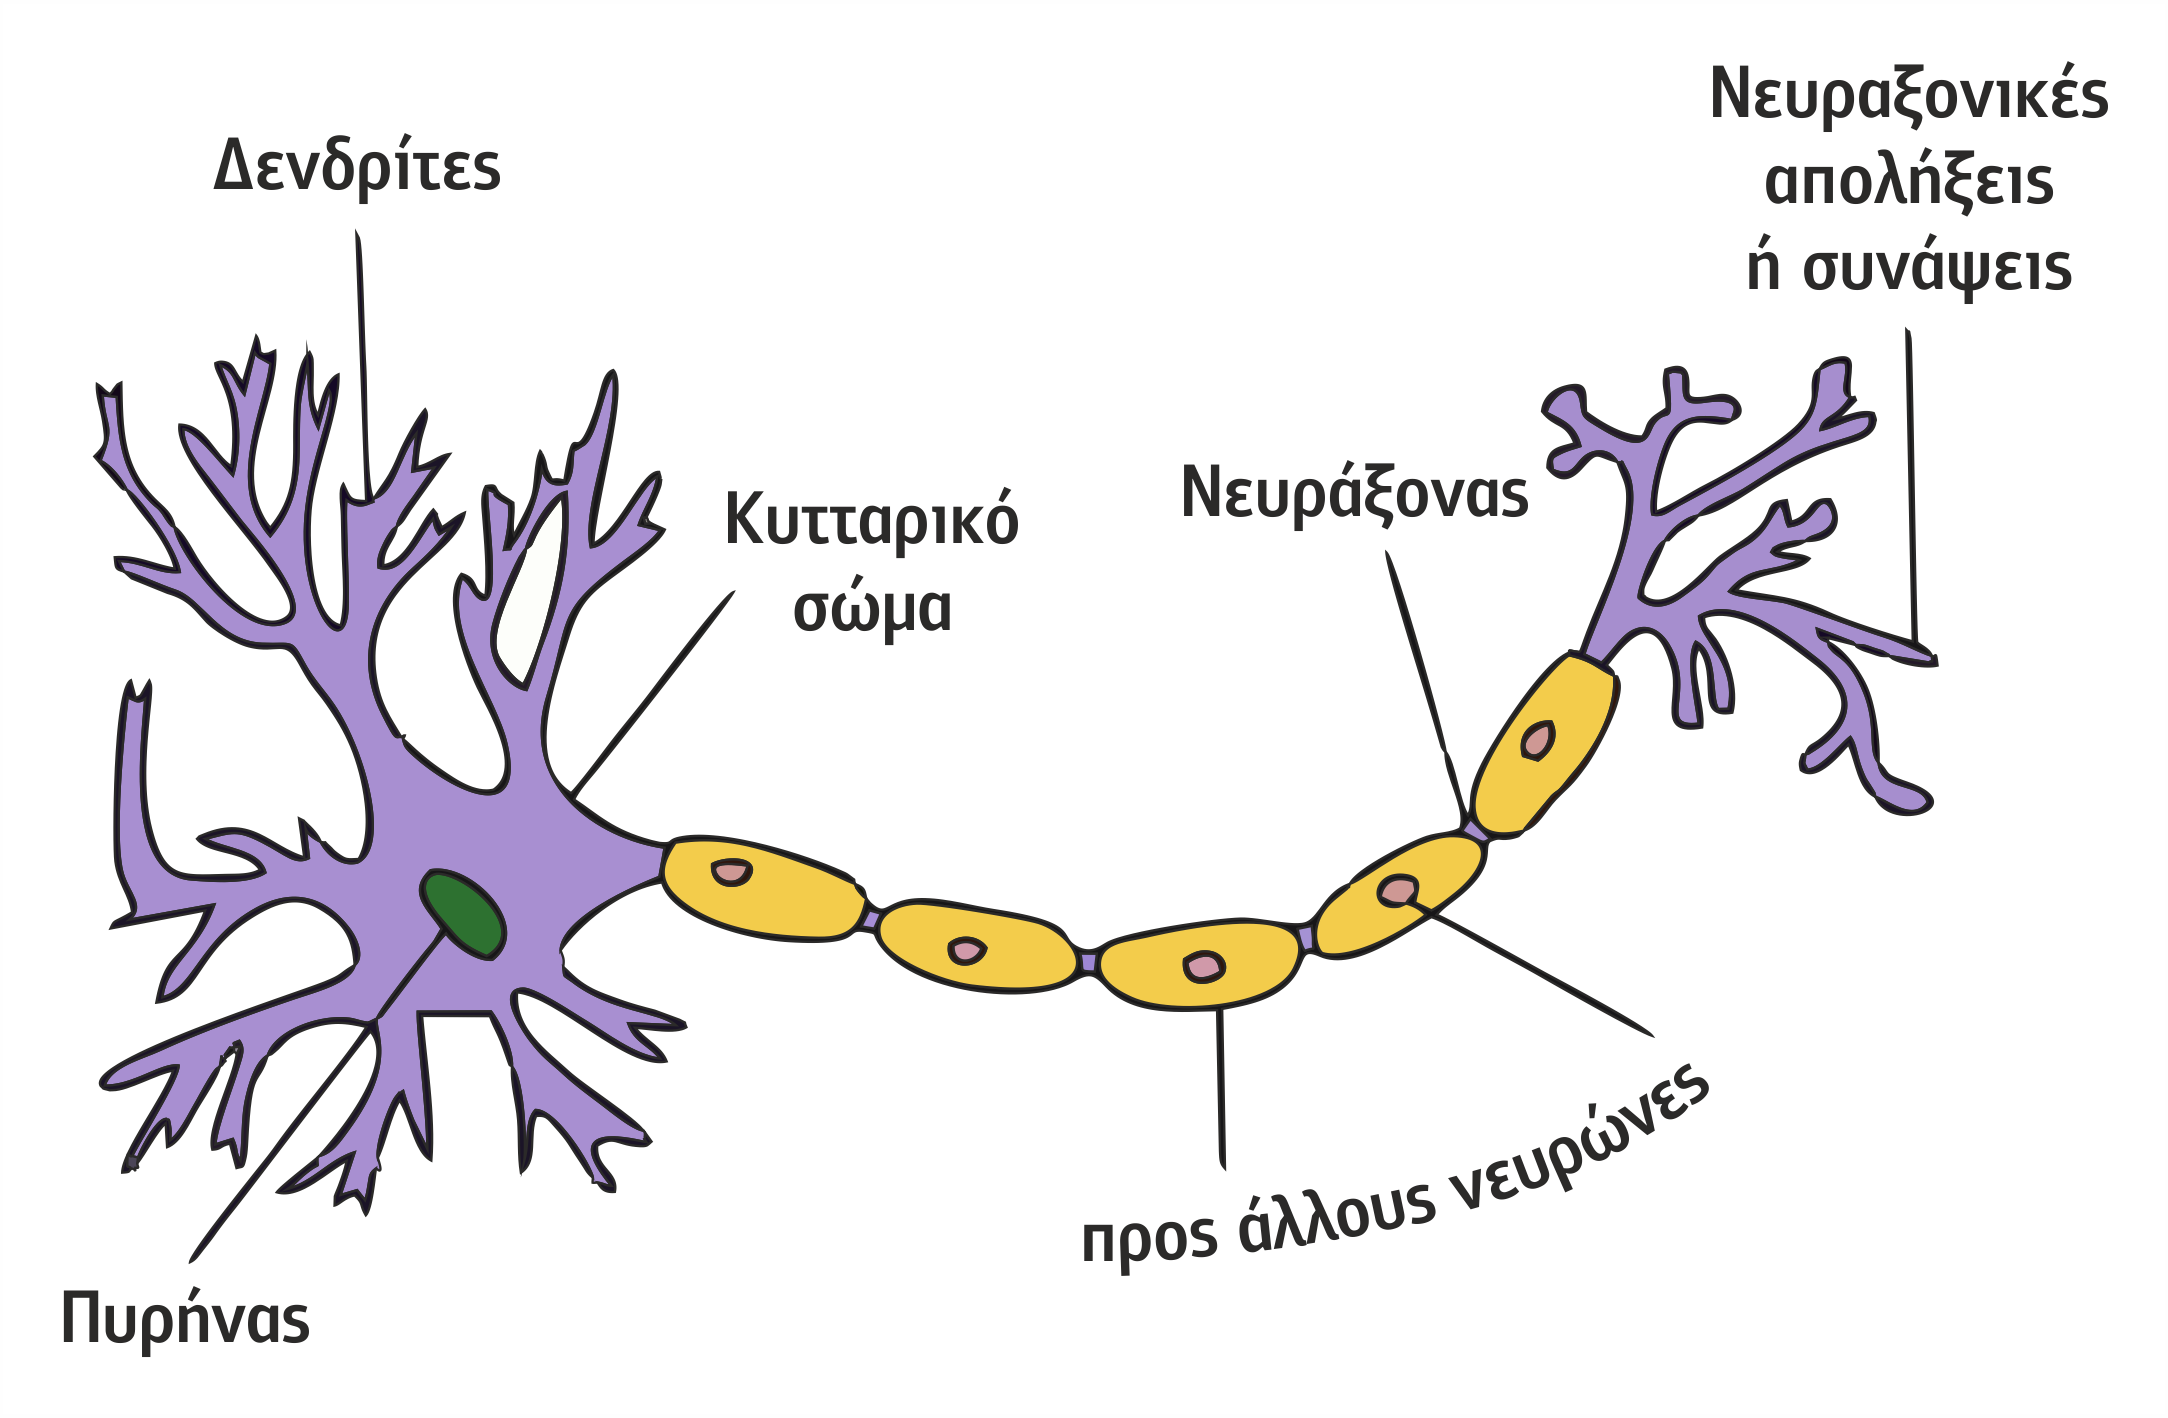
\includegraphics[width=0.7\textwidth]{./images/chapter3/neuron.png}
  \caption[Βιολογικός Νευρώνας]{Βιολογικός νευρώνας.}
  \label{fig:neuron_bio}
\end{figure}
Στο \autoref{fig:neuron_bio} φαίνεται η μορφή και tα μέλη ενός βιολογικού νευρώνα
Τα κύρια μέρη ενός νευρώνα είναι τα εξής:
\begin{itemize}
  \item{\textbf{Δενδρίτης (Dendrites)}: Δέχεται είσοδο από άλλους νευρώνες.}
  \item{\textbf{Σώμα του κυττάρου (Cell body)}: Εξάγει συμπεράσματα, με βάση τις εισόδους.}
  \item{\textbf{Νευράξονας (Axon)}: Συνδέει την έξοδο που λαμβάνεται από το σώμα του κυττάρου με τις νευρωνικές απολήψεις}
  \item{\textbf{Νευραξονικές απολήψεις}: Συνδέει τον νευράξονα του εκάστοτε νευρώνα με τους τερματικόυς κόμβους
    από όπου και μεταφέρεται η πληροφορία σε άλλους νευρώνες.
    είσοδο άλλων νευρώνων.}
\end{itemize}
Κάθε νευρώνας δέχεται είσοδο από άλλους νευρώνες μέσω των δενδρίτων του.
Στην συνέχεια επεξεργάζεται το σήμα που λαμβάνει στην είσοδο και
στέλνει το αποτέλεσμα στον νευράξονα. Τέλος άλλοι νευρώνες συνδέονται με αυτόν
μεσω των συνάψεων του.

\begin{figure}[!ht]
  \centering
  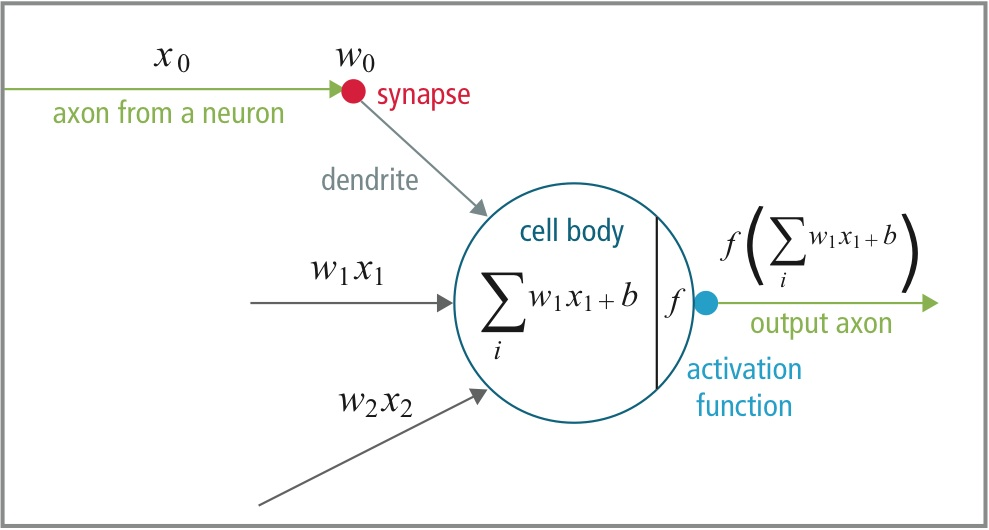
\includegraphics[width=0.7\textwidth]{./images/chapter3/neuron_model.jpg}
  \caption[Μαθηματικό μοντέλο του νευρώνα]{Μαθηματικό μοντέλο του νευρώνα}
  \label{fig:neuron_model}
\end{figure}

To αντίστοιχο μαθηματικό μοντέλο του νευρώνα, φαίνεται στο \autoref{fig:neuron_model}.
H πληροφρία που μεταφέρεται από τις νευραξονικές απολήψεις ($x0$), πρωτού
στους δενδρίτες των επόμενων νευρώνων, αλληλεπιδρά πολλαπλασιαστικά με τις
συνάψεις ($w0*x0$). Oι πολλαπλασιστικοί παράγωντες $w_n$ ονομάζονται βάροι
και αποτελούν τις μεταβλητές παραμέτρους ενός νευρώνα. Η τιμή των παραμέτρων
αυτών ελέγχουν την επίδραση μεταξύ των νευρώνων. Η συνάρτηση ενεργοποίησης $f$
ελέγχει την ροή της πληροφορίας στους συνδεδεμένους νευρώνες,
και προσδίδει ευελιξία και ικανότητα εκτίμησης όσον αφoρά πολύπλοκες μή γραμμικές
σχέσεις στα δεδομένα εισόδου.
Η πιο συχνά χρησιμοποιούμενη και απλή στην λειτουργία συνάρτηση ενεργοποίησης
είναι η σιγμοειδής συνάρτηση $\sigma(x) = 1 / (1 + e^{-x})$.
Εναλλακτικά, η σιγμοειδές συνάρτηση ενεργοποίησης μπορει να εκφραστει σε διακριτή μορφή ως
\[
f(x) =
  \begin{cases}
    0, & x < 0 \\
    1, & x \geq 0 \\
  \end{cases}
\]
Η επιλογή εφαρμογής της σιγμοειδής συνάρτησης, ως συνάρτηση ενεργοποίησης των
νευρώνων δεν είναι τυχαία, αφού όπως θα δούμε στην
συνέχεια επιτρέπει την χρησιμοποίηση του αλγορίθου \emph{Backpropagation} για την
εκπαίδευση των νευρωνικών δικτύων.

Γενικότερα, ο νευρώνας μπορεί να είναι και πολωμένος (bias - $b$) και έτσι το μαθηματικό
μοντέλο που τον περιγράγει πλήρως παίρνει την μορφή:
\begin{center}
\begin{large}
  $\sigma = f(\sum_{\imath} \vec{X_{\imath}}\vec{W_{\imath}} + b) = \frac{1}{1 + e^{-\sum_{\imath} \vec{X_{\imath}}\vec{W_{\imath}} + b}}$
\end{large}
\end{center}
Θα μπορούσαμε να ερμηνεύσουμε το αποτέλεσμα της εφαρμογής της
σιγμοειδή συνάρτηση ενεργοποίησης ώς την πιθανότητα μίας από τις κλασεις:
\begin{center}
\begin{large}
  $P(y_{\imath} = 1 | x_{\imath};w)$ \\
  $P(y_{\imath} = 0 | x_{\imath};w) = 1 - P(y_{\imath} = 1 | x_{\imath};w)$
\end{large}
\end{center}

Σαν παρατήρηση, με εφαρμογή κατάλληλης
συνάρτησης σφάλματος στην έξοδο, ο νευρώνας μετατρέπεται σε ένα  γραμμικό ταξινομητή
(linear classifier). Πιο συγκεκριμένα, σε περίπτωση που χρησιμοποιήσουμε την \emph{cross-entropy}
συνάρτηση σφάλματος ο νευρώνας μετατρέπεται σε δυαδικό ταξινομητή \textbf{Softmax},
τον οποίο και θα συναντήσουμε στην συνέχεια.

\begin{figure}[!ht]
  \centering
  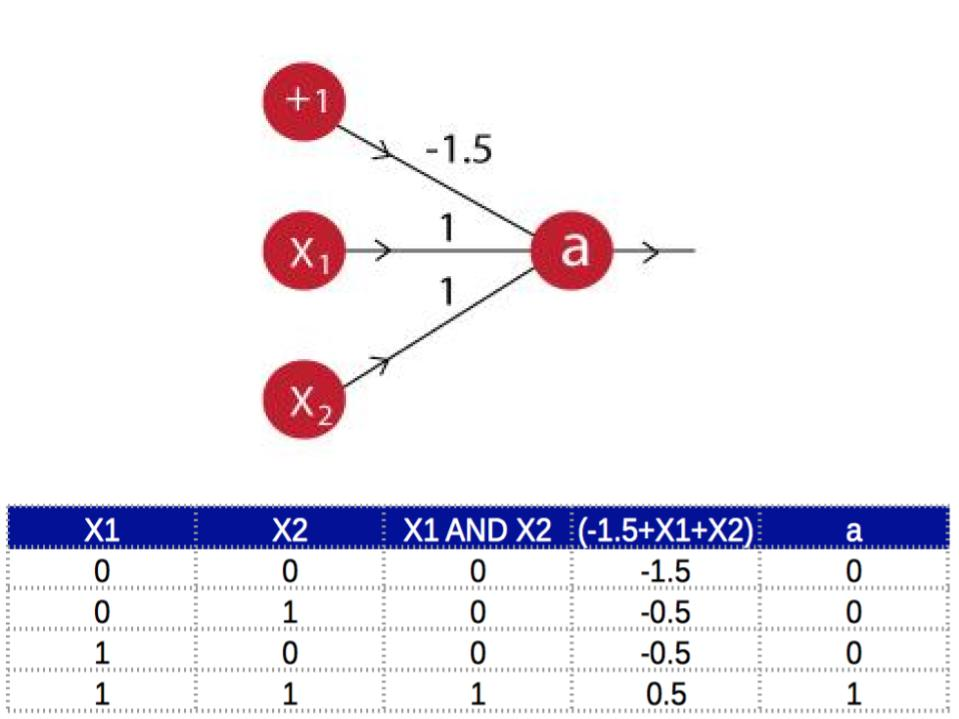
\includegraphics[width=0.6\textwidth]{./images/chapter3/perceptron_and.jpg}
  \caption[Υλοποίηση πύλης AND με χρήση του μαθηματικού μοντέλου του νευρώνα]{Υλοποίηση πύλης AND με χρήση του μαθηματικού μοντέλου του νευρώνα}
  \label{fig:neuron_and}
\end{figure}

Οι τρεις θεμελιώδη εφαρμογές τoυ μαθηματικού μοντέλου του νευρώνα είναι οι
μονtελοποίηση των λογικώ πυλών \emph{AND, OR και NOT}. Στο \autoref{fig:neuron_and}
παρουσιάζeται το αντίστoιχο μοντέλο της λογικής πύλης \emph{AND}. Ο νευρώνας
δέχεται σαν είσοδο 2 σήματa ($X_{1}$,  $X_{2}$) και μία παράμετρο πόλωσης ($b=-1.5$).
Η έξοσος $a$ ορίζεται ως:
\[
  a = f(x) = f(X_{1}, X_{2}) =
  \begin{cases}
    0, & x < 0 \\
    1, & x \geq 0 \\
  \end{cases},  
  όπου x = X_{1} + X_{5} - 1.5
\]

H σύνδεση πολλών νευρώνων σε σε έναν γράφο δομεί ένα \emph{Νευρωνικό Δίκτυο}.
Το μοντέλο ΝΝ που φαίνεται στο \autoref{fig:simple_nn}
ονομάζεται \emph{Perceptron} ή αλλιώς
\emph{Feedforward Artificial Neural Network - ANN}, ο οποίος έχει τα εξής χαρακτηριστικα:
\begin{itemize}
  \item{Οι διασυνδέσεις μεταξύ των νευρώνων δεν σχηματίζουν σε καμία περίπτωση κύκλο.}
  \item{Αποτελείτε από 2 επίπεδα; ένα κρυφό και το επίπεδο εξόδου}
  \item{Χρησιμοποιείται η σιγμοειδή συνάρτηση ενεργοποίησης}
\end{itemize}
Ονομάζεται Feedforward γιατί η πληροφορία ρέει προς μία μόνο κατεύθυνση, δηλαδή
η έξοδος νευρώνα στο $\imath$ επίπεδο δεν συνδέεται με την είσοδο νευρώνα
που βρίσκεται το επίπεδο $k \leq \imath$.
To Perceptron δέν είναι το μόνο
μονέλο ΝΝ που ανήκει στην κατηγορία των Feedforward ANN. Όπως θα δούμε στο
\autoref{sec:theory_cnn}, τα \emph{Νευρωνικά Δίκτυα Συνέλιξης
(Convolutional Neural Networks - CNN)} ανήκουν και αυτά στην κατηγορία αυτή.

\begin{figure}[!ht]
  \centering
  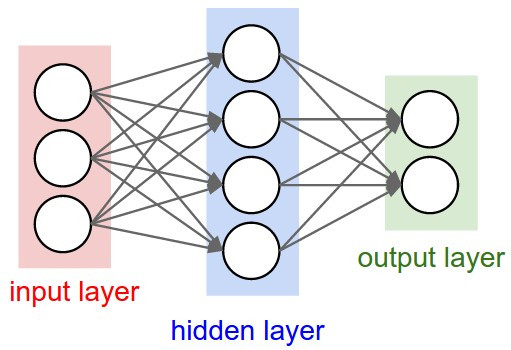
\includegraphics[width=0.5\textwidth]{./images/chapter3/simple_nn.jpg}
  \caption[Απλό μοντέλο NN με ένα κρυφό επίπεδο - Perceptron]{Απλό μοντέλο NN με ένα κρυφό επίπεδο - Perceptron}
  \label{fig:simple_nn}
\end{figure}

H γενική (δισδυάστατη) δομή ενός νευρωνικού δικτύου φαίνεται στο \autoref{fig:multilayer_nn}.
Τα γνωρίσματα ενός τέτοιου, \emph{πολυ-επίπεδου ΝΝ)}, είναι τα εξής:
\begin{itemize}
  \item{Αριθμός κρυφών επιπέδων}
  \item{Αριθμός των νευρώνων στο κάθε επίπεδο}
\end{itemize}
Η έξοδος από το κέθε επίπεδο μπορεί να εκφραστεί ως
\[
  A_{\imath+1} = f_{\imath}(A_{\imath} \bullet W_{(\imath)} + B_{\imath}), \\
  A_{\imath} = M \times N, W_{\imath} = K \times M, B_{\imath} = K \times N
\]
όπου η τιμή του $\imath$ αναφέρεται στον αριθμό.
O αριθμός των επιπέδων, ή καλύτερα το μέγιστο μήκος του μονοπατιού που ακολουθεί
η πληροφορία από την είσοδο μέχρι την έξοδο του ΝΝ, ορίζει το \emph{βάθος} ενος ΝΝ.

\begin{figure}[!ht]
  \centering
  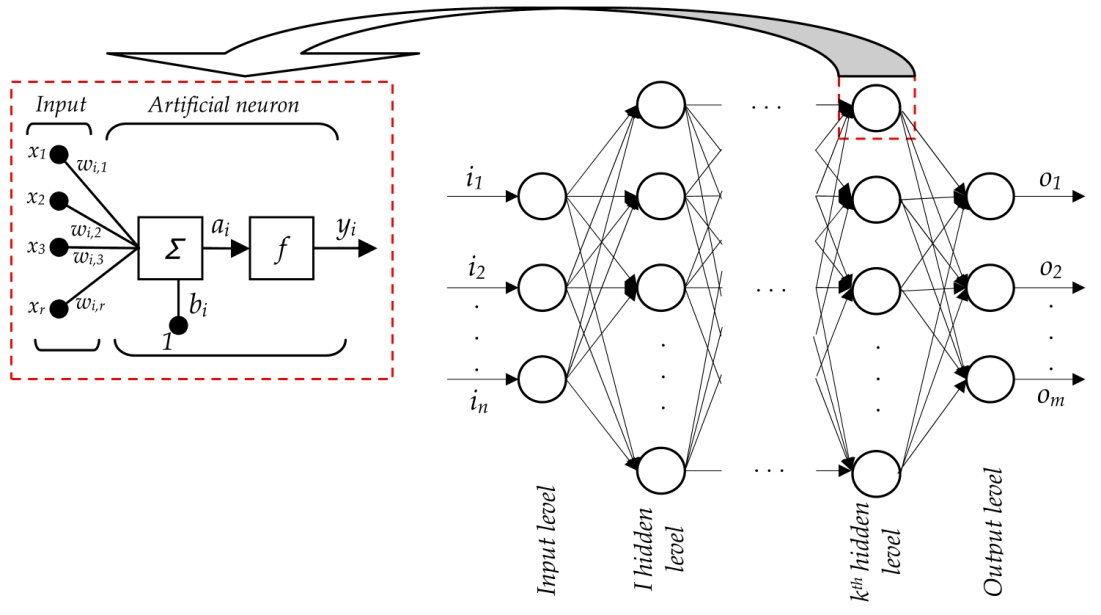
\includegraphics[width=0.6\textwidth]{./images/chapter3/multilayer_nn.jpg}
  \caption[Απλό μοντέλο NN με ένα κρυφό επίπεδο - Perceptron]{Απλό μοντέλο NN με ένα κρυφό επίπεδο - Perceptron}
  \label{fig:multilayer_nn}
\end{figure}

\begin{algorithm}[!htp]
  \caption{Feedforward αλγόριθμος}
  \label{alg:nn_forward}
  \begin{algorithmic}[1]
    \Function{activation}{a}
      \State \Return $1.0 / (1.0 + e^{-a})$
    \EndFunction \\
    \Procedure{nn\_forward}{X, W, B, num\_layers}
      \State Starting from the input layer, use $\sigma$ to do
         a forward pass trough the network, computing the activities of the
        neurons at each layer.
      \State $k \gets 0$
      \While{$k < num\_layers$}
      \State $X^{k} \gets \Call{activation}{X \bullet W_{k} + B_{k}}$  \Comment{If we want to keep output from
        intermediate layers, we must add up one dimension on $X$}.
        \State $k \gets k+1$
      \EndWhile
    \EndProcedure
  \end{algorithmic}
\end{algorithm}

O \autoref{alg:nn_forward} υλοποιεί την διαδικασία για τον υπολογισμό της εξόδου
ενός νευρωνικού δικτύου (forward pass), έχοντας σαν δεδομένα τα βάρη και τις τιμές της πόλωσης
των νευρώνων του κάθε επιπέδου, καθώς και τα δεδομένα εισόδου.


\subsection{Συναρτήσεις Ενεργοποίησης}

\textbf{Σιγμοειδές - Signmoid} \\

Η συγμοειδές μή γραμμική συνάρτηση έχει την μορφή που είδαμε στην αρχή του κεφαλαίου.
\[
  \sigma(x) = 1 / (1 + e^{-x})
\]
Παίρνει σαν είσοδο έναν πραγματικό αριθμό και τον κανονικοποιεί στο διάστημα $[0, 1]$

\begin{figure}[!ht]
  \centering
  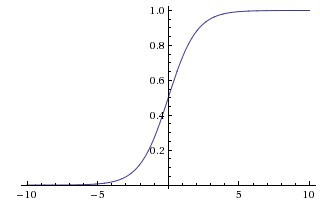
\includegraphics[width=0.4\textwidth]{./images/chapter3/sigmoid.jpg}
  \caption[Συνάρτηση Σιγμοειδούς συνάρτησης]{Συνάρτηση Σιγμοειδούς συνάρτησης}
  \label{fig:sigmoid}
\end{figure}

\textbf{Υπερβολική Εφαπτωμένη - Tanh} \\

Παίρνει σαν είσοδο έναν θετικό αριθμό και τον κανονικοποιεί στο διάστημα $[-1, 1]$.
\[
  \tanh{x} = 2\sigma(2x) - 1
\]

\begin{figure}[!ht]
  \centering
  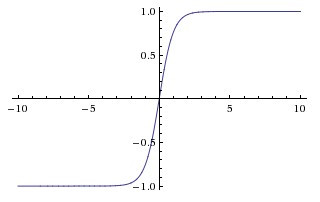
\includegraphics[width=0.4\textwidth]{./images/chapter3/tanh.jpg}
  \caption[Συνάρτηση Υπερβολικής Εφαπτωμένης]{Συνάρτηση Υπερβολικής Εφαπτωμένης}
  \label{fig:tanh}
\end{figure}

\textbf{ReLU} \\

Μία από τις πιο δημοφιλές συναρτήσεις ενεργοποίησης τα τελευταία χρόνια.
Πρακτικα κρατά την ενεργοποίηση οριοθετημένη στο μηδέν και είναι
γρήγορη στον υπολογισμό.
\[
  f(x) = \max(0, x)
\]

\begin{figure}[!ht]
  \centering
  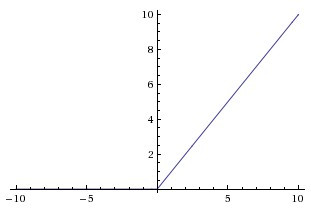
\includegraphics[width=0.4\textwidth]{./images/chapter3/relu.jpg}
  \caption[Συνάρτηση Rectified Linear Unit - ReLU]{Συνάρτηση Rectified Linear Unit - ReLU}
  \label{fig:tanh}
\end{figure}

Το μειονέκτημά της είναι ότι κατά την διάρκεια της εκπεύδευσης του νευρωνικού
δικτύου τα βάρη να ανανεώνονται με τέτοιο τρόπο που ο νευρώνας να μην ενεργοποιηθεί
ποτέ. Αυτό έχει σαν αποτέλεσμα να "σκοτώσει" τον εκάστωτε νευρώνα.

\textbf{Leaky ReLU} \\

\textbf{Maxout} \\

\subsection{Αλγόριθμος Stochastic Gradient Descent}
TODO!

\subsection{Αλγόριθμος Backpropagation}

Ο αλγόριθμος \emph{backpropagation} εμφανίστηκε το 1970, και υποτιμήθηκε
μέχρι το 1986, όταν και οι David Rumelhart, Geoffrey Hinton, και Ronald Williams
απέδειξαν την αποδοτικότητα του στην εκπαίδευση των νευρωνικών δικτύων, κυρίως
όσον αφορά στην ταχύτητα \cite{rumelhart1988learning}.
Πλέον χρησιμοποiείται για την εκαπίδευση
μεγάλων νευρωνικών δικτύων με εκατομμύρια παραμέτρους.

Αυτό που προσπαθεί να καταφέρει ο αλγόριθμος \emph{backpropagation} είναι να
ελαχιστοποιήσει το σφάλμα, δωσμένης μίας συνάρτησης σφάλματος. Υπολογίζει
το σφάλμα και ανανεώνει ανάλογα τις τιμές του πολυ-επίπεδου νευρωνικού δικτύου.

Μία συνάρτηση σφάλματος έχει την γενική μορφή:
\[
  E_{total} = f(target - output)
\]


\subsection{Αρχιτεκτονικές}

TODO!
